\documentclass[12pt,a4paper]{article}

\usepackage[left=3cm, right=3cm, top=2.5cm, bottom=2.5cm]{geometry}
\usepackage{setspace}
\usepackage{amsmath}
\usepackage{tikz}
\usepackage{pgfplotstable}
\usepackage{titlesec}
\usepackage{bm}
\usepackage{tcolorbox}
\tcbuselibrary{skins}
\usepackage{empheq}

\titleformat{\section}{\Large\bfseries}{\thesection}{1em}{}
\titleformat{\subsection}{\large\bfseries}{\thesubsection}{1em}{}

\renewcommand{\contentsname}{Table des Matières}
%\renewcommand{\baselinestretch}{1.5}

\title{Étude du Pendule Simple : Analyse des Oscillations Harmoniques}
\author{Cătălin Bozan, Liviu Arsenescu}
\date{05.03.2024}

\newtcbox{\mymath}[1][]{%
    nobeforeafter,
    math upper,
    tcbox raise base,
    enhanced,
    colframe=black,
    colback=white,
    boxrule=1pt,
    drop shadow={
        shadow xshift=3pt,
        shadow yshift=-3pt,
        opacity=1
    },
    #1
}

\begin{document}
    \pagenumbering{gobble}
    \begin{titlepage}
        \begin{center}
            \vspace*{\fill}
            \Huge \textbf{Étude du Pendule Simple :} \\
            \Huge \textbf{Analyse des Oscillations Harmoniques} \\
            \Large Rapport du Laboratoire \\
            \vspace{\fill}
            \Large Cătălin Bozan, Liviu Arsenescu \\
            05.03.2024

            \vspace*{\fill}
        \end{center}
    \end{titlepage}
    \newpage

    \pagenumbering{arabic}
    \section{Objectifs du laboratoire}
    \begin{itemize}
        \item Démontrer expérimentalement le fait que la période ne dépend pas de la masse
        \item Vérifier la formule de la période d'un pendule
        \item Trouver l'accélération gravitationnelle de la terre
    \end{itemize}

    \section{Éléments théoriques}
    \subsection{Les différentes quantités rencontrées}
    \begin{itemize}
        \item $\bm{\theta}$ - l'angle entre la verticale et le pendule
        \item \textbf{L} - la longueur du fil
        \item \textbf{T} - la période du pendule
        \item \textbf{m} - masse d'objet
        \item \textbf{s} - la position de la masse
        \item \textbf{g} - l'accélération gravitationnelle
    \end{itemize}
    \subsection{La formule fondamentale du pendule}
    La position de la masse suspendue est calculée à l'aide de la formule suivante: 
    \begin{equation*}
        s=L\theta,
    \end{equation*}
    La deuxième loi de Newton ($\sum_{i=1}^{n} F_i=ma$) selon l'axe tangentiele s'écrit:
    \begin{equation*}
        -mgsin(\theta) = m\frac{d^2s}{dt^2}
    \end{equation*}
    où $-mgsin(\theta)$ est l'équation obtenue pour la seule force agissant sur l'objet (P - poids), et $\frac{d^2s}{dt^2}$ est l'accélération totale du système, obtenue en dérivant deux fois la position. \\
    On sait que $\frac{d^2s}{dt^2} = L\frac{d^2\theta}{dt^2}$ (L - constante). Alors:
    \begin{align*}
        -mgsin(\theta)&=mL\frac{d^2\theta}{dt^2} \\
        -\frac{g}{L}sin(\theta)&=\frac{d^2\theta}{dt^2} \\
        \frac{d^2\theta}{dt^2}+\frac{g}{L}sin(\theta)&=0
    \end{align*}
    Pour notre expérience, nous n'utilisons que de petits angles, ce qui nous permet de faire l'approximation suivante: $sin(\theta) \approx \theta$. Le pendule simple devient alors un système oscillatoire harmonique, décrit par l'équation suivante:
    \begin{empheq}[box={\mymath}]{equation*}
        \frac{d^2\theta}{dt^2}+\frac{g}{L}\theta=0
    \end{empheq}
    En comparant cette équation avec l'équation du mouvement oscillatoire harmonique ($\frac{d^2x}{dt^2}+\omega^2x(t)=0$), nous obtenons:
    \begin{empheq}[box={\mymath}]{gather*}
        \omega=\sqrt{\frac{g}{L}} \\
        T=\frac{2\pi}{\omega}=2\pi\sqrt{\frac{L}{g}}
    \end{gather*} 
    Cette approche mathématique permet de tirer les conclusions suivantes:
    \begin{itemize}
        \item La période ne dépends pas de la masse de l'objet
        \item La période est proportionnelle à la raacine carrée de la longueur
        \item Nous pouvons estimer expérimentalement la norme d'accélération gravitationnelle à l'aide de la formule: 
        \begin{equation*}
            g=\frac{4\pi^2L}{T^2}
        \end{equation*}
    \end{itemize}   

    \section{Manipulation}
    
    %figure pendule
    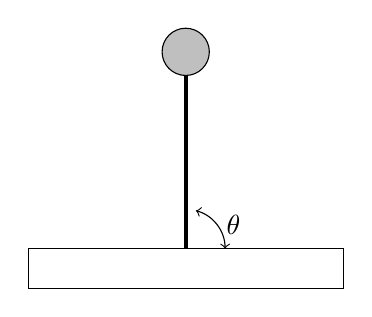
\begin{tikzpicture}
        % Table
        \draw (0, 0) rectangle (4, 0.5);
        
        % String
        \draw (2, 0.5) -- (2, 3);
        
        % Pendulum bob
        \filldraw[fill=gray!50, draw=black] (2, 3) circle (0.3);
        
        % Pendulum rod
        \draw[line width=1.5pt] (2, 0.5) -- (2, 2.7);
        
        % Angle notation
        \draw[<->] (2.5, 0.5) arc (0:75:0.5) node[midway, right] {$\theta$};
    \end{tikzpicture}

    \section{Mesures}

    \section{Analyse des mesures et résultats}

    \section{Synthèse et conclusion}
\end{document}

